%TODO: obviously rewrite this
In this section I will explain what I've done and the stack used for this thesis: I will start by reviewing the OpenFace tool (\ref{OpenFace}), the database (\ref{rldb}) utilized and all the experiments and techniques used, such as.....

%TODO: pipeline OPENFACE + analysis. here or architecture?
%TODO: SHORT review (table pherhaps) of face db, maybe not in this section

\section{OpenFace} \label{OpenFace}
The OpenFace \cite{Baltru2018} toolkit is a tool for machine learning and computer vision researchers created ba Baltrusaitis et al. to perform facial landmark detection, head pose estimation, action unit recognition and eye gaze estimation. \\

\begin{figure}[H]
	\centering
	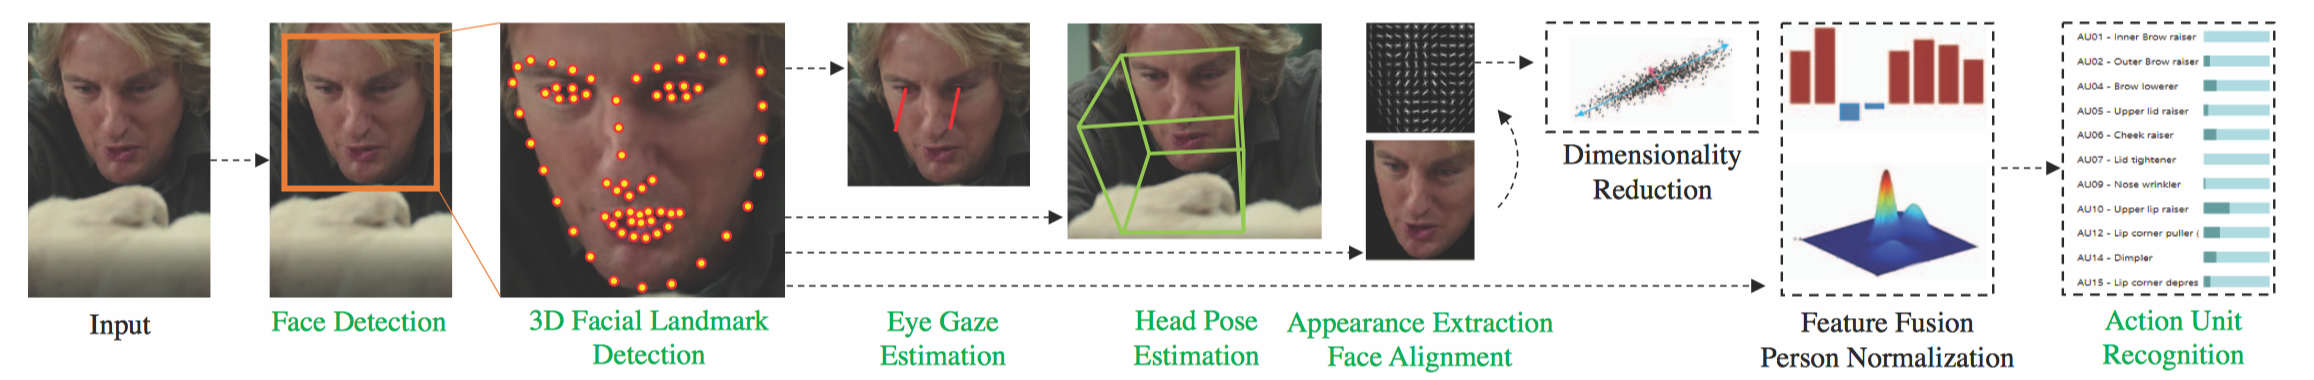
\includegraphics[width=1\textwidth]{openface20_pipeline}
	\caption{OpenFace Pipeline \cite{Baltru2018}}
	\label{fig:openface20_pipeline}
\end{figure}

\subsection{Landmark Detection}
The first step in Action Unit identification is to detect the facial landmarks. To accomplish this a local detector called Convolutional Experts Network (CEN) \ref{fig:CEN} is utilized. CEN has the advantage of aggregating a neural architecture and patch experts (local detectors, they evaluate the probability of a landmark being aligned at a particular pixel location). CEN can learn different patch experts and adapt to diverse appearance models without explicit attribute labeling. \\

\begin{figure}[H]
	\centering
	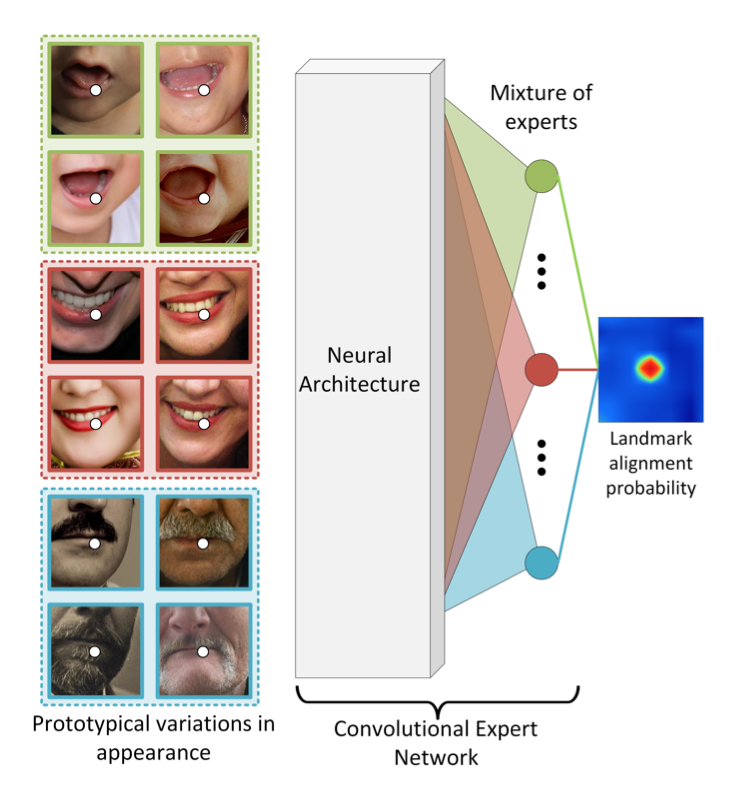
\includegraphics[width=0.5\textwidth]{CEN}
	\caption{Facial landmarks naturally cluster around appearance prototypes (facial hair, expressions, make-up etc). To model such appearance variations a Convolutional Experts Network (CEN) is used to bring together the advantages of neural architectures and mixtures of patch experts to model landmark alignment probability. \cite{Baltru2017}.}
	\label{fig:CEN}
\end{figure}

%TODO: write better?
OpenFace uses a Convolutional Experts Constrained Local Model (CE-CLM) \cite{Baltru2017}, which is a Constrained Local Model (CLM) that uses CEN as a local detector. CLM are used to model the appearance of each facial landmark individually by using local detectors and a shape model for constrained optimization.\\
The CE-CLM is divided in two fundamental parts: response map computation using CEN, and shape parameter update. In the first step, the landmarks alignment is computed separately from the other landmarks. In the second phase, all landmarks are considered together and for misaligned landmarks and irregular shapes their position is penalized, using a Point Distribution Model (PDM).\\

\subsubsection{CEN}
In the first step the objective is to generate a response map to localize the individual landmarks. This is achieved by assessing the landmark alignment probability at specific pixel locations. CEN takes in input a Region of Interest (ROI) around the currently estimated position of a landmark, and outputs a response map that calculates the landmark alignment probability at each pixel location (Fig. \ref{fig:landmark_det}). \\
\begin{figure}[H]
	\centering
	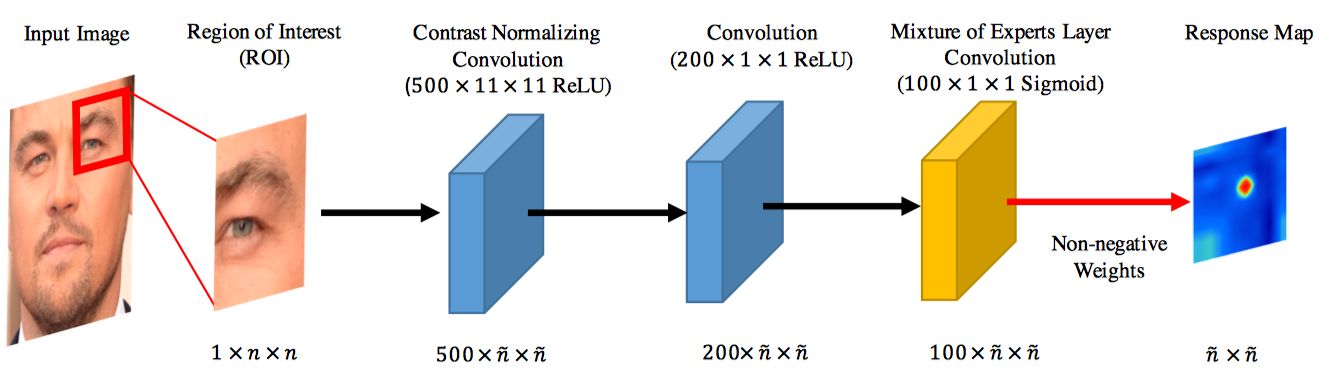
\includegraphics[width=1\textwidth]{landmark_det}
	\caption{Overview of the Convolutional Experts Network model. The output response map is a non-negative and non-linear combination of neurons in ME-layer using a sigmoid activation \cite{Baltru2017}.}
	\label{fig:landmark_det}
\end{figure}
%TODO: to specific?
In order to do all this, the ROI is initially passed in a Contrast Normalizing Convolution layer to perform z-score normalization and to calculate the correlation between input and kernel. The output is then convolved in another layer of ReLU neurons (convolution is an operation on two functions to produce a third function that expresses how the shape of one is modified by the other). \\
The last neural layer before the response map is the Mixture of Expert Layer (ME-layer), and it can model the alignment probability using a combination of patch experts (local detectors) that are able to represent different landmarks appearance prototypes by outputting individual votes on alignment through a sigmoid function. The response maps from all the local detectors are then combined in the final layer, giving a final alignment probability.

\subsubsection{Point Distribution Model}
The point distribution model is a used to represent the mean geometry of a shape and some statistical modes of geometric variation inferred from a training set of shapes \cite{wiki:PDM}. Point distribution models rely on landmark points. \\
First, a set of training images are manually landmarked with enough corresponding landmarks to sufficiently approximate the geometry of the original shapes.
Then the shape outlines are reduced to sequences of k landmarks, so that a given training shape is defined as the vector $\mathbf {X} \in \mathbb {R} ^{2k}$.
 The matrix of the top d eigenvectors is given as $\mathbf {P} \in \mathbb {R} ^{2k\times d}$, and each eigenvector describes a principal mode of variation along the set.
 Finally, a linear combination of the eigenvectors is used to define a new shape $ \mathbf {X} '$, mathematically defined as:
 
 $ \mathbf {X} '={\overline {\mathbf {X} ))+\mathbf {P} \mathbf {b} $ where $ {\overline {\mathbf {X} ))}$ is defined as the mean shape across all training images, and $\mathbf {b}$  is a vector of scaling values for each principal component. Therefore, by modifying the variable$ \mathbf {b}$  an infinite number of shapes can be defined. 
														
Point Distribution Models is employed in the second phase of the algorithm, and have two objectives: they are used to control the landmark locations, and to regularize the shape in the CE-CLM framework. Irregular shapes for final detected landmarks are penalized.
PDM models the location of facial feature points in the image using non-rigid shape and rigid global transformation parameters. The appearance of local patches around landmarks of interest is modelled using patch experts. The fitting strategies employed in CLMs are varied, a popular example is the Regularised Landmark Mean Shift (RLMS). Once the model is trained on labelled examples, a fitting approach is used to estimate the rigid and non-rigid parameters p, which fit the underlying image best:




















\section{Real Life Trial DataBase} \label{rldb}

\section{GLM}

\section{LDA}

\section{QDA}

\section{SVM}

\section{Correlations} ?